\documentclass{article}
\usepackage[utf8]{inputenc}
\usepackage{graphicx}
\title{Early Detection of Infectious Disease with Smartwatch Data}
\author{Andreas Ink}
\date{March 2022}

\usepackage{comment}

\newcommand\todo[1]{\textcolor{blue}{#1}}
\usepackage{todonotes}
\usepackage{biblatex} %Imports biblatex package
\addbibresource{easy.bib}
\begin{document}

\maketitle
\section{Abstract}


This report is designed to examine prior research and propose improvements to such research on detecting COVID-19 with smartwatches.  Prior research such a study conducted by Stanford University and their algorithm NightSignal, achieved 78\% accuracy when predicting COVID-19 via heart rate.  While impressive, the accuracy may be improved, including improvements suggested by the study by outlining various factors to improving future research.  These factors include adding heart rate variability, respiration rate, blood oxygen, among other physiological data points.  The core rational for pursuing this research (Vito) is to reduce spread of COVID-19, to increase algorithm usage by encouraging trust in a community via ambitious privacy standards and community involvement and to create a more efficient and convenient on-device algorithm.  The primary method to examine the efficiency of the algorithm was comparing the results of NightSignal to Vito, treating NightSignal as the actual result and Vito as the predicted result.  This resulted in 99.9\% accuracy when comparing the two algorithms. This is significant as people use technology that's easy to use and works, thus, the faster the algorithm can run and return a result the more people will use it and reduce the spread of COVID-19.  Further, the algorithm can run in the background and send stress event alerts in the background, therefore, reducing the need to check the app daily, thus increasing algorithm usage to reduce the spread of COVID-19.

\section{Introduction}

COVID-19 is an infectious disease that has impacts everyone particularly during waves.  During such waves there are two major issues, testing becomes less accessible and people may be asymptomatic, thus not receive a test and sequentially isolate.  Studies show Covid-19 may be detectable with physiological markers such as heart rate~\cite{NightSignal}, heart rate variability~\cite{hrv}, and respiration rate~\cite{vital}. Smartwatches can collect this data and detect changes in physiological markers to alert of infectious disease.  While a personal story, my Aunt had an immunocompromised immune system and had Covid-19.  While she survived the infection, she died months later due to other causes, prior to infection, others around her were displaying symptoms, thus if a tool to contentiously monitor physiological markers, my Aunt could have received more treatment faster or isolated from the family members who displayed symptoms to possibly improve her quality of life and lifespan.  

Vito is an app and possible research study with the goals of reducing spread of COVID-19 via physiological derived alerts, to encourage trust in a community via ambitious privacy standards and community involvement, and to increase app usage with greater convenience via a more efficient on-device algorithm that utilizes smartwatch data to detect COVID-19 in real time. Vito is heavily based on a study conducted by Stanford University and the algorithm created from the study, NightSignal~\cite{NightSignal}. NightSignal has a 78\% accuracy when predicting COVID-19 with heart rate data while asleep.  Further, the study determined that COVID-19 stress related alerts occurred for a mean of 4.9 days, compared to 1.9 days for non-COVID stress alerts.  The study also details how to possibly improve accuracy of future algorithms, primarily adding additional physiological based data.  Notably, some of NightSignal alerts were associated with vaccination.  A newer study with an algorithm, CovidDeep~\cite{coviddeep}, utilizes neural networks and novel data points such as blood oxygen, and respiration rate.  The accuracy of this model is 98\%, which is significantly higher than NightSignal's 78\%. 

\section{Methodology}
Vito is an app and future research study with the goal of early infectious disease detection using physiological data commonly collected with smartwatches.  This section is designed to outline Vito's data collection and processing, goals, and overall experimental setup.
% \todo{Restate what Vito is above and briefly introduce the outline of the subsections. (short intro)} 

\subsection{Model}
The computation, a deterministic finite state machine is heavily derived from the study mentioned in the above section. The state machine operates on levels, with each level having conditions to increase or decrease a level. Further illustration of the model and pipeline in figure~\ref{fig:model}.  As stated previously in the report, the computations are on-device rather than on a server, thus the setup required a few challenges.  Notably, mass data processing was challenging due to memory constraints, however, this was resolved by testing the bulk data in a macOS app rather than an iOS app.  The Android app faces a similar issue and is not yet resolved.  Additionally, configuring Apple's HealthKit database was problematic to an extent as it required optimization, while the Fitbit health database is easier to work with, albeit, Vito has limited Fitbit support as of March 15, 2022.  The state machine's accuracy was calculated assuming the study cited above is the true value and Vito is the predicted value. Separately, the informal vaccination analysis was analyzed with a machine learning model and will be further evaluated with a state machine in the future.  

% \todo{reduce color and add more input and output, black box around model, arrows for input and output}
\begin{figure}

\begin{center}
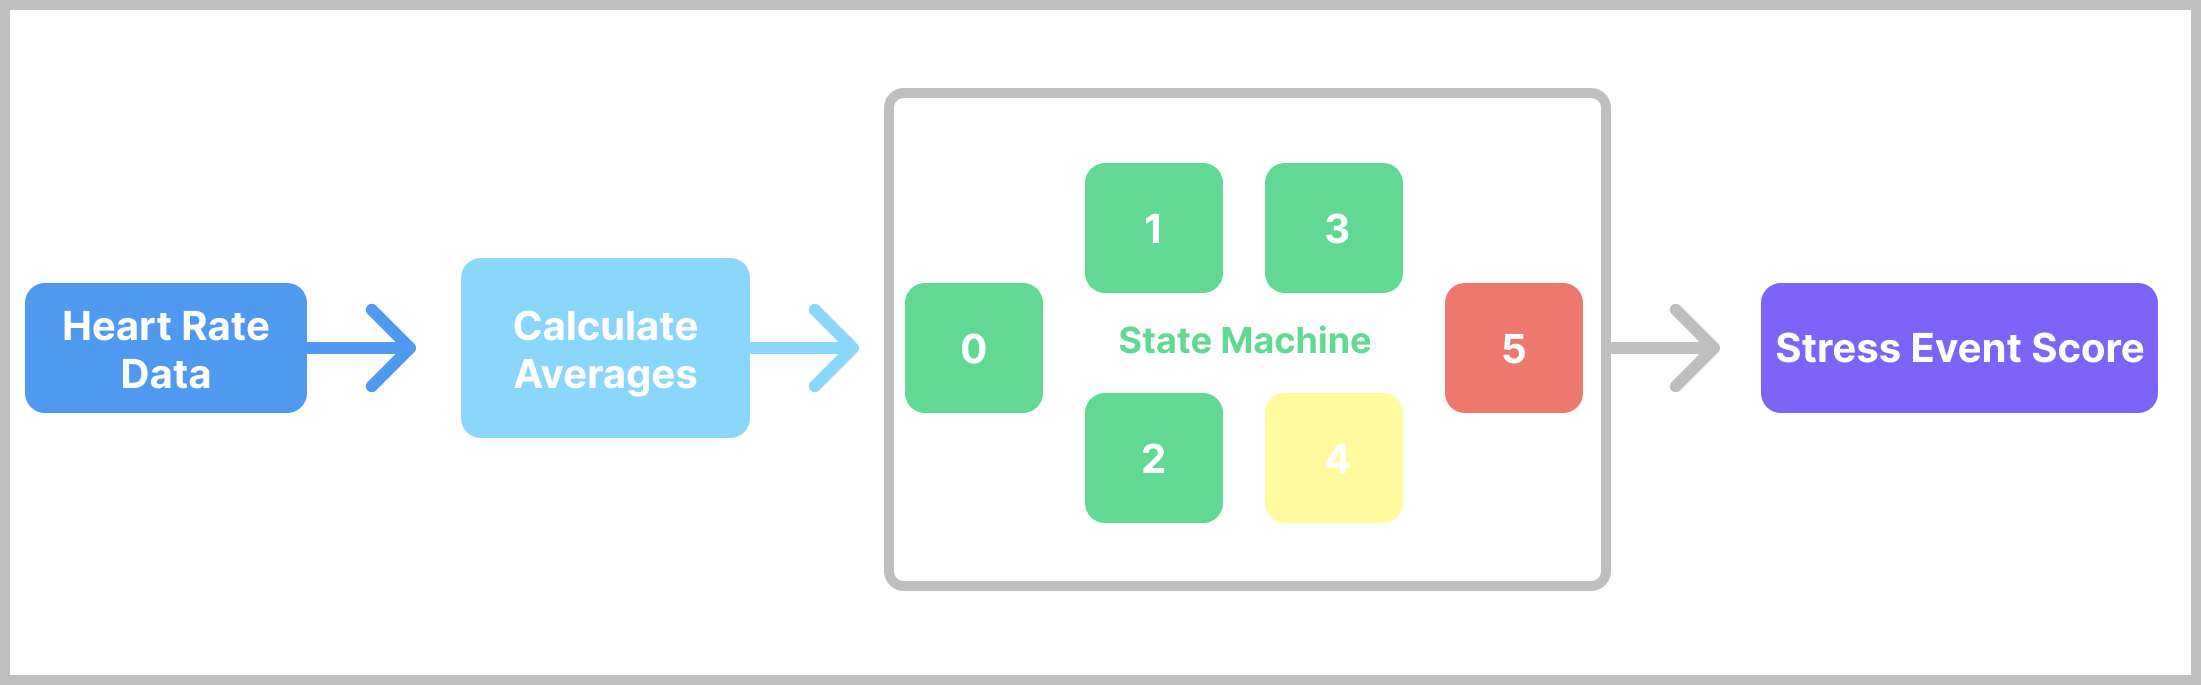
\includegraphics[scale=0.15]{VitoPipeline.png}
\end{center}
\caption{
Vito's model pipeline for iOS, from data collection to the state machine}
\label{fig:model}
\end{figure}


Below, we will focus on the three main aspects of improvement over NightSignal~\cite{NightSignal}: (1) Algorithmic Efficiency, (2) Reduce Spread, and (3) Encourage Trust.


% \todo{Make sure to refer to it within text at least one time. use \label and \ref tags to refer to fig within text.}
% \todo{I think there is still something wrong with how you are placing figures, you may be missing parenthesis or tags, see here: "Captioning, labelling and referencing" of "Inserting Images" in the overleaf guide, both figures (keyword figures)}

\subsubsection{Algorithmic Efficiency}
Efficiency of an algorithm directly correlates to app usage as people will use technology if it is easy and quick to use, therefore, accomplishing Vito's first goal, reducing the spread of COVID-19. An on-device algorithm is more efficient as it circumvents the time intensive process of uploading data to a server for processing.  This translates to three major advantages, the ability to process data in the background to send alerts without the participant entering the app after onboarding, increased privacy, therefore, trust due to the absence of exporting data, and significantly faster computation time that increases the convenience to the participant.  Notably, recent updates to asynchronous code in Swift and filtering the heart rate data based on activity associated with the heart rate value enabled faster processing.  

\subsubsection{Reduce Spread}
While the app can not directly advise a participant to receive a COVID-19 test, isolate, or give any other medical advice in compliance with IRB, Vito may state that the previous night indicates there may have been a stress event.  A stress event classifies as a significant increase in heart rate and respiratory rate, lower heart rate variability and blood oxygen levels.  Thus, the participant can choose to take action on the alert, such as testing for COVID-19 while not being directed explicitly to get tested to comply with IRB protocol. According to the National Institutes of Health (NIH), "A positive test early in the course of the illness enables individuals to isolate themselves – reducing the chances that they will infect others and allowing them to seek treatment earlier, likely reducing disease severity and the risk of long-term disability, or death."~\cite{nih}  Additionally, if Vito has a similar effect as exposure notifications on the outcome of a pandemic, infections would at least decline by 4\% at 15\% community adoption.~\cite{en}  However, Vito's adherence to progressive privacy standards and other suggested measures to increase adoption will likely lead to further adoption.  Therefore, if an app such as Vito, can be utilized to encourage further testing, a positive test would encourage isolation, therefore reducing the spread of COVID-19 to others.

\subsubsection{Encourage Trust}
Health data can be particularly sensitive for many despite appropriate privacy and security measures.  As I learned from working on Covid Watch~\cite{covidwatch}, an exposure notification app originally built by a team of volunteers, some will only use technology if it is safe, secure, effective, convenient, and has a human element.  The core issue as to why Covid Watch did not reach adequate adoption rates was primarily due to its effectiveness, lack of community involvement, and human connection.  
From our point of view, this can be established via overall community engagement, such as involving as many people in the community as possible in the app.  Secondly, being present in the community is critical, such as addressing problems people face in a non-technical way that still addresses problems posed by the pandemic such as increased economic hardship that may be improved by community food drives.  Additionally, open sourcing the software may be important to establishing trust and also optimizing feedback and overall app quality.  Additionally, Vito clearly states what data it imports (Fitbit health data) and exports (none), and proves this by displaying instructions on how to access one's privacy report conducted by Apple on iPhone's.

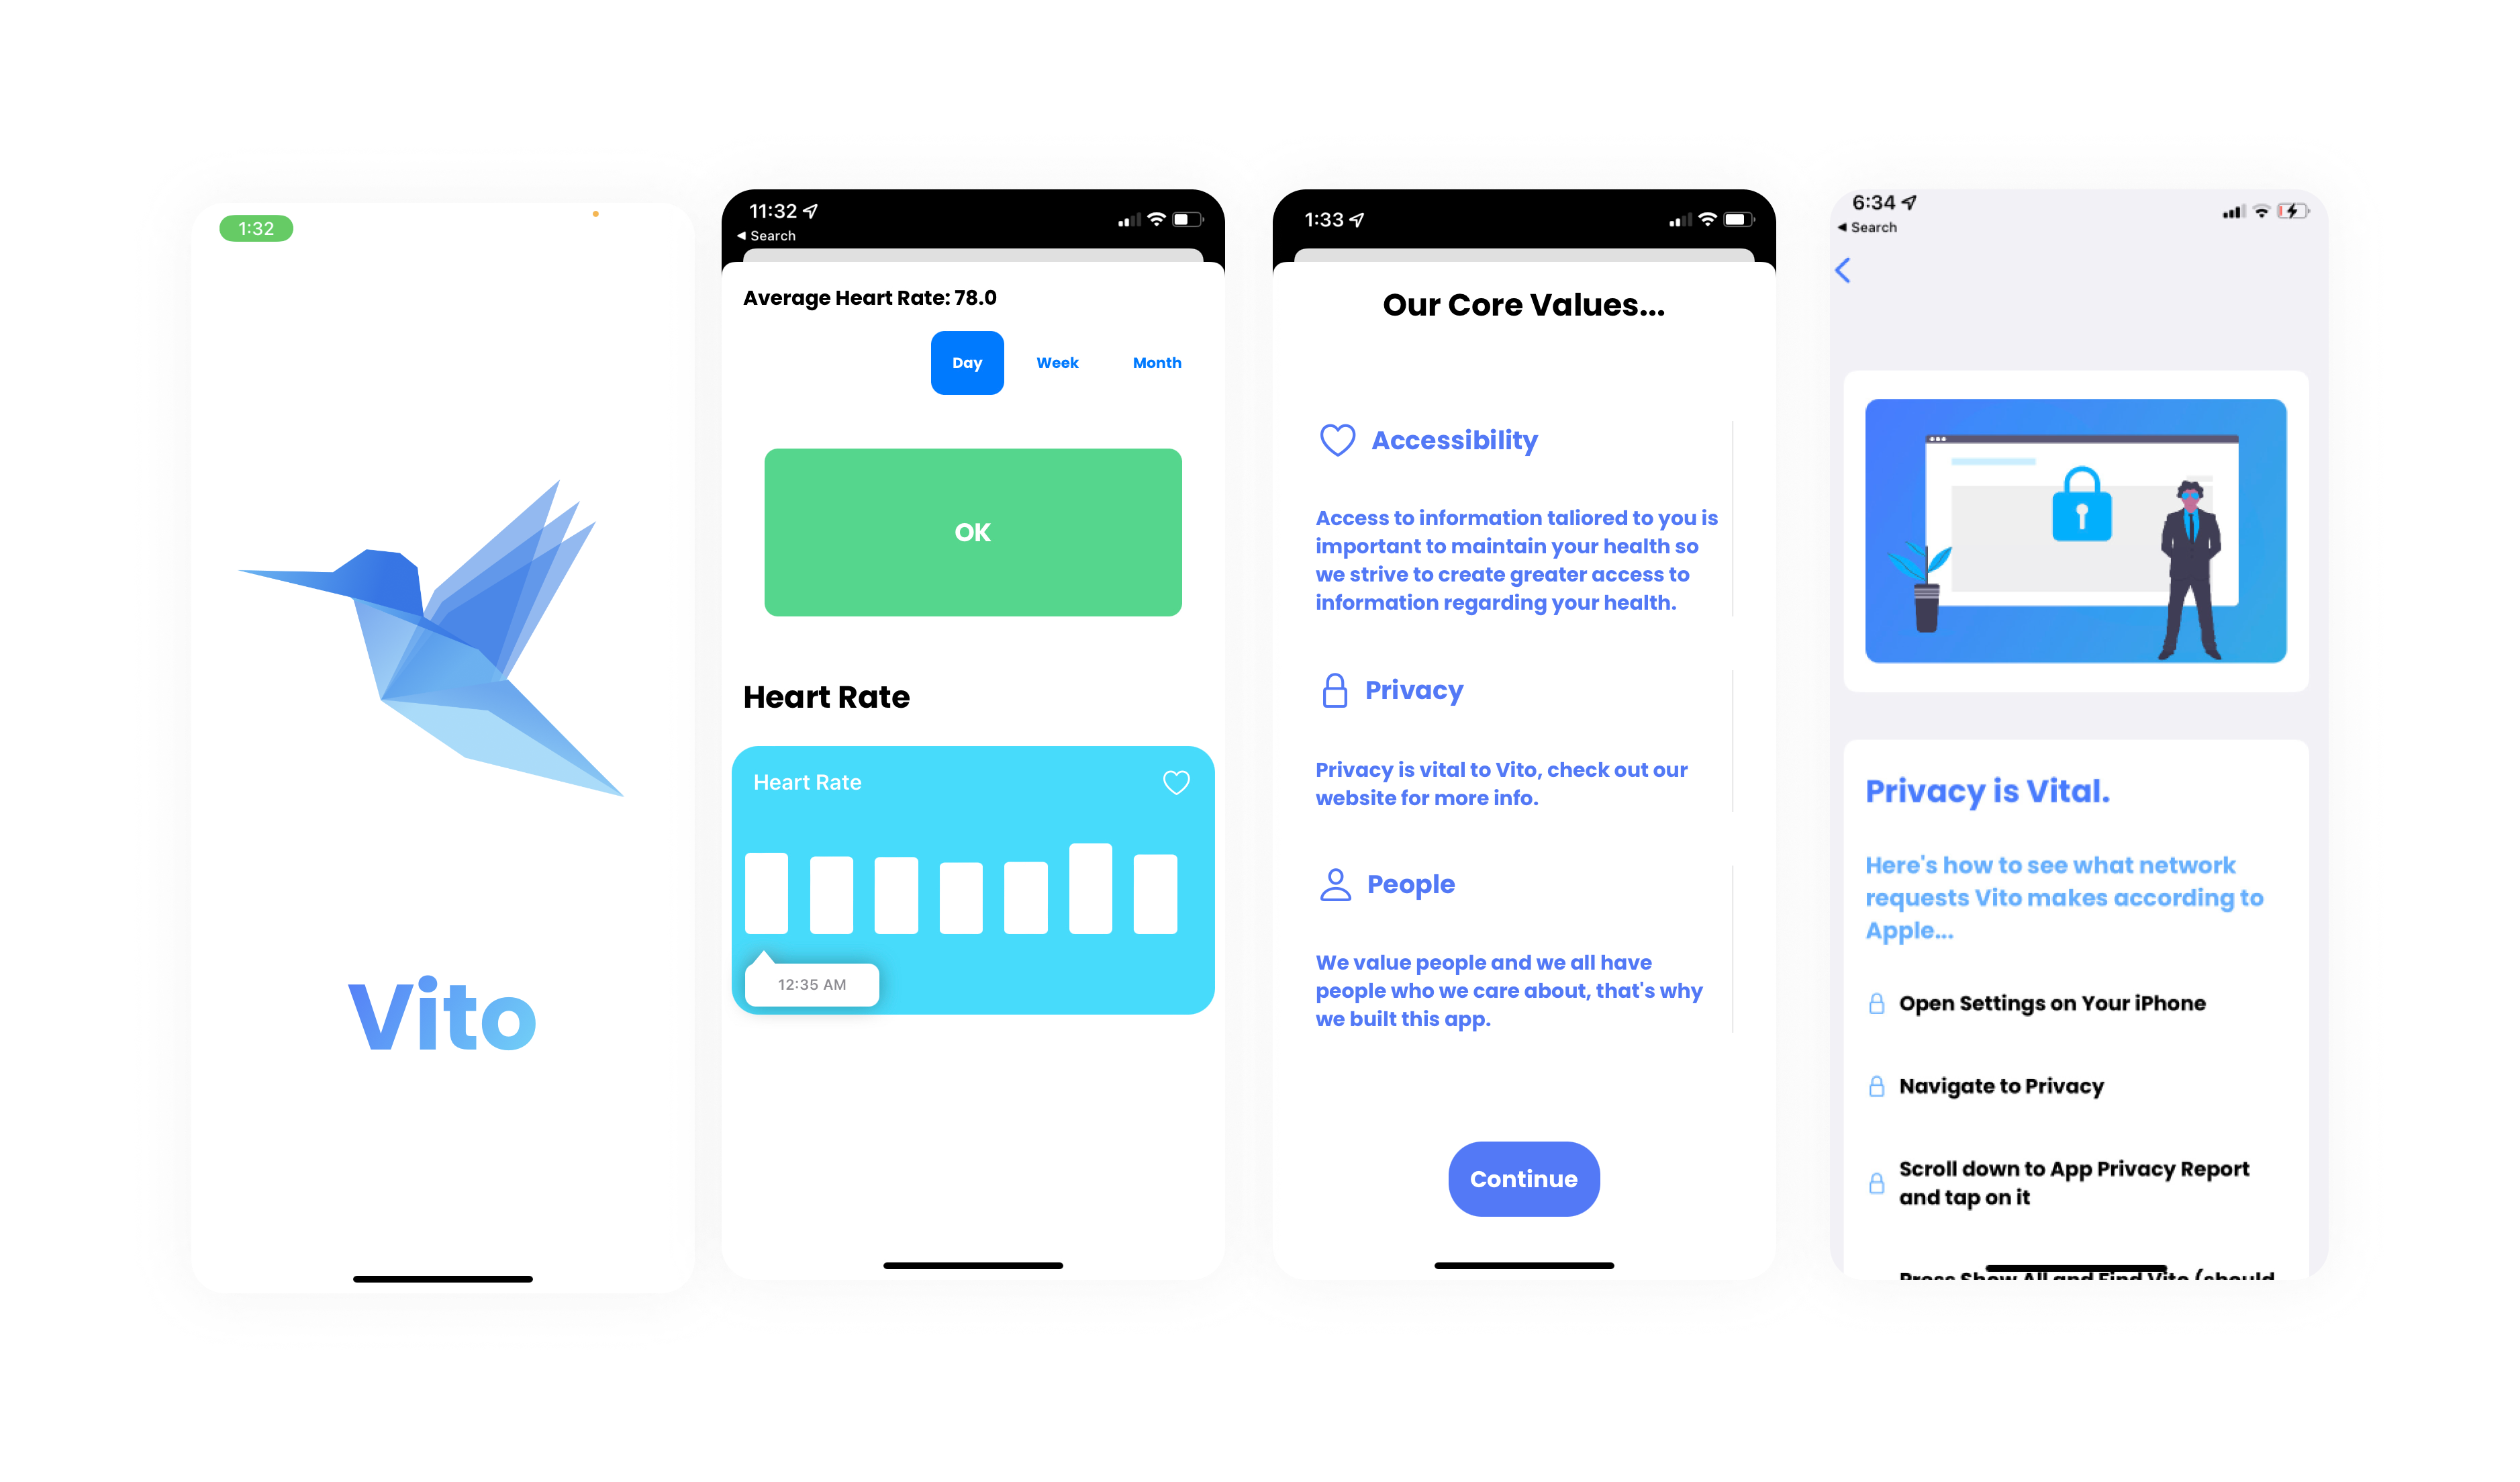
\includegraphics[scale=0.08]{VitoApps.png} 

\caption{
Views from Vito's iOS app that shows Vito's loading view, data details, a view from on-boarding, and privacy policy}

\subsection{Data}
The data examined includes 3,246 number of participants' unidentified heart rate and step data derived from NightSignal, preliminary/informal data collected following a Moderna COVID-19 booster vaccine among one participant~\cite{VaccineData}, and data following an non-Covid-19 infection~\cite{VitoAnalysis}.  The methodology of examining one participant's data following vaccination was to examine various new metrics such as heart rate variability, ECG readings, and respiration rate as NightSignal determined that vaccination may cause a similar physiological response as infection of COVID-19.

% \todo{use nonbreaking space, i.e. ~ before /cite commend}

 \footnote{

Vito's Data: 

https://github.com/Vito-Research/Vito-Analysis

NightSignal's Data:  

https://storage.googleapis.com/gbsc-gcp-project-ipop_public/COVID-19-Phase2/COVID-19-Phase2-Wearables.zip
}
% \todo{add links using footnote tag}

\subsection{Experimental Setup}
Data sets include open sourced heart rate and step data from the NightSignal study, health data collected from the time period in which I was sick, and my health data after my vaccination.  Metrics utilized include Kappa score~\ref{fig:kappa}, precision, recall~\ref{fig:acc}, and overall accuracy.  We treated NightSignal as if it were the actual value and Vito as the predicted value, thus treating it as a machine learning validation.  Each metric scored 99.9\% with test accuracy.  Regarding performance metrics, we utilized a simple stopwatch to calculate the time from launch to viewing the infection risk score on NightSignal's app myPHD and Vito's app.  We look to further improve on the performance metrics by analyzing how different computational techniques impact app performance. 
% \todo{talk about the specific datasets, validation techniques and performance metrics you used for comparing Vito to NightSignal. (add more, stats, people, define scores (math equation tag), add validation (test data set)}

\begin{figure}
        P_o &= \frac{1}{N} \sum_{j = 1}^k f_{jj}, \\
        r_i &= \sum_{j = 1}^k f_{ij}, \forall i, \text{ and }
        c_j = \sum_{i = 1}^k f_{ij}, \forall j, \\
        P_e &= \frac{1}{N^2} \sum_{i = 1}^k r_i c_i,

\label{fig:kappa}
\caption{
Kappa Score}
\end{figure}

\begin{figure}
     Precision = \frac{TP}{TP+FP}
     Recall = \frac{TP}{TP+FN}

\label{fig:acc}

\caption{
Precision and Recall Scores}
\end{figure}




\section{Results and Discussion}
When comparing NightSignal~\cite{NightSignalGithub} and Vito's computations in Swift (iOS), the accuracy of Vito is 99.9\% accurate, with a kappa score, recall, and precision higher or equal to 99.9\%~\cite{VitoAnalysis}.  With Kotlin, a programming language for Android, the accuracy is 89\%.  This may be for a few reasons, a novice misunderstanding of Kotlin, a data import error that is evident in some files, regardless, the accuracy needs to be increased and further examined.  Further, algorithmic efficiency was increased by three minutes (Vito - 2 minutes and 30 seconds, NightSignal 6+ minutes) on iOS by comparing the duration from app launch to alert results when querying 3 months of data. When comparing data (heart rate variability and respiration rate) prior to vaccination and shortly after vaccination, the informal results were roughly 70\% accurate in predicting vaccination assuming the stress event lasted up to two days after vaccination.  Additionally, while examining my health data 3 days prior to symptom onset of non-COVID respiratory illness and prior, my heart rate over night increased by 12 BPMs, heart rate variability decreased by 11.5 ms, respiration rate increased by 2 BPMs, energy burned increased by 0.1 calories.  These changes may be due to increased stress leading up to and during infection.  Please note, that the symptoms appeared on week 12 (the last week in the charts below).
%\subsection{

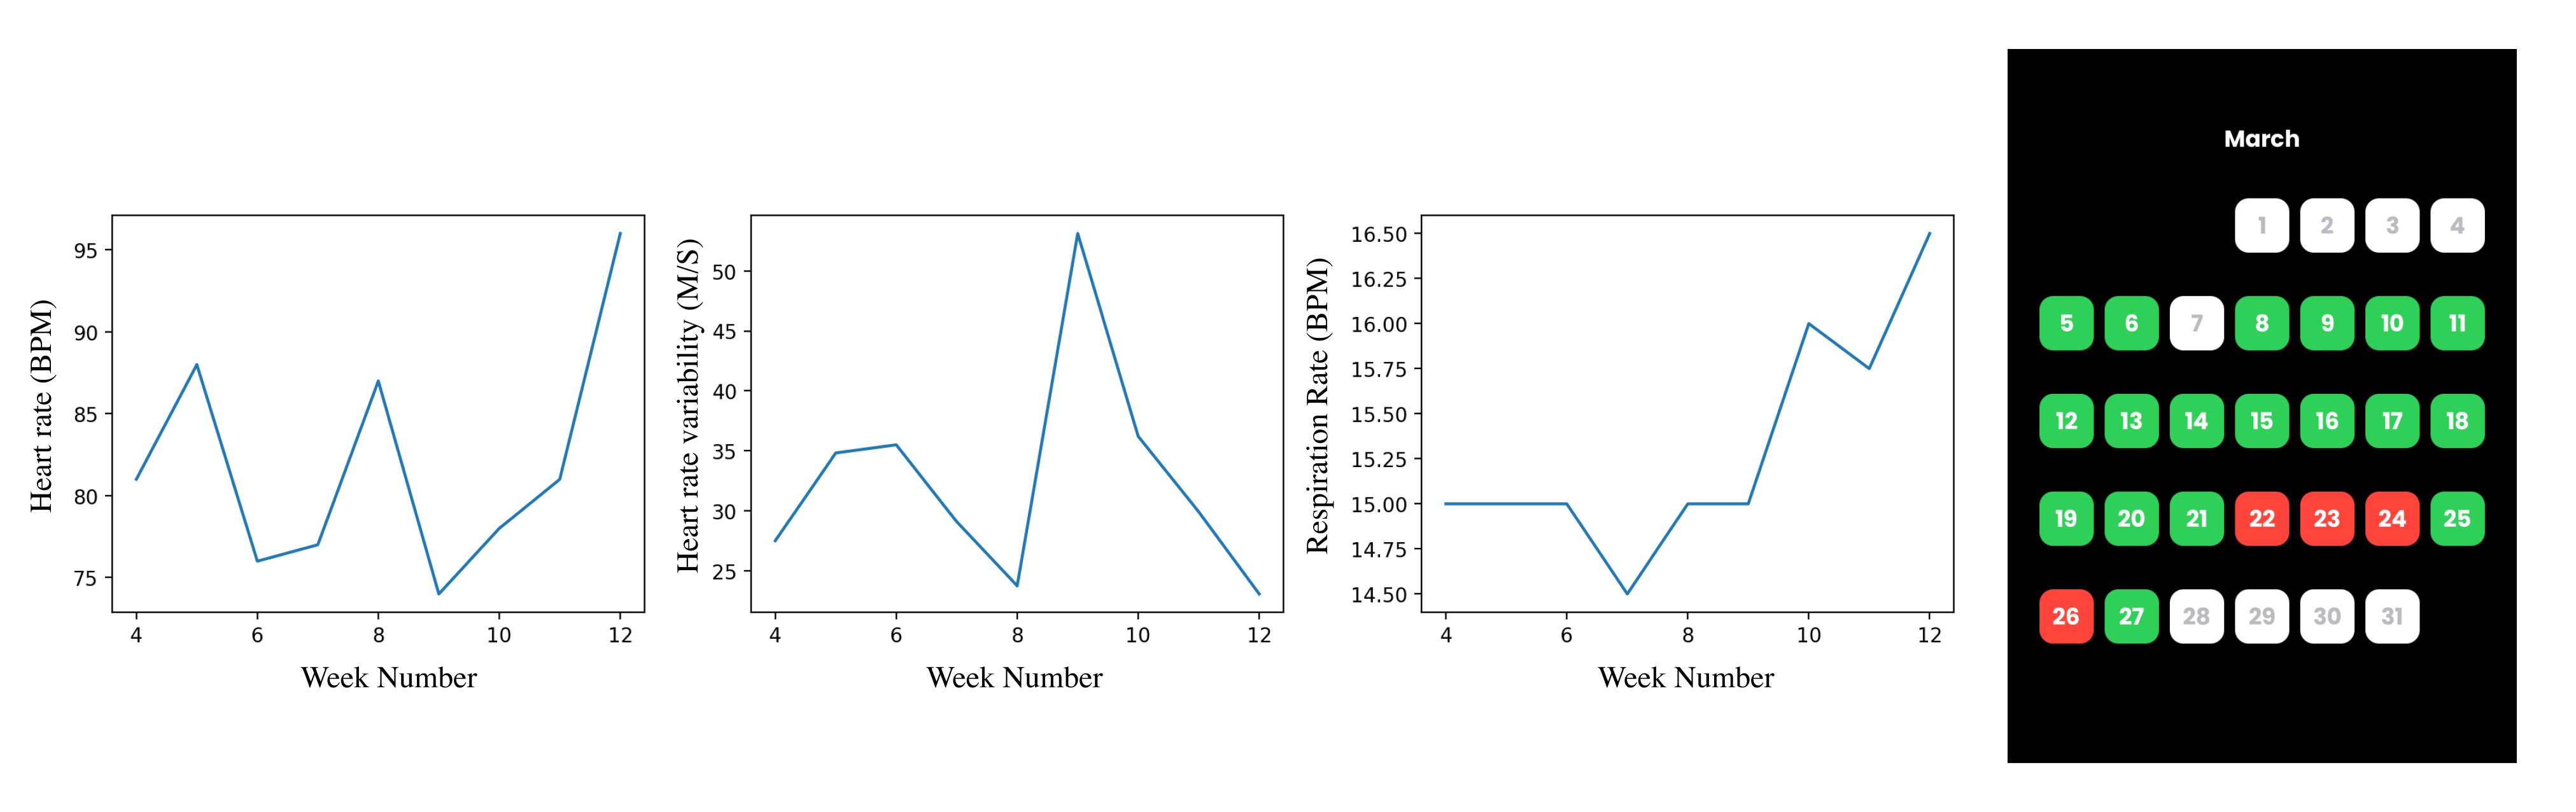
\includegraphics[scale=0.07]{VitoInfo.png}

\caption {
(Charts) Heart rate, heart rate variability, and respiration rate. 
(App Graphic) Alerts leading up to symptoms on the 25th of March, the third day of alerts
}

%}

% \todo{hard to read the plot text, subplots}

\section{Conclusion and Further Research}
 This report discussed Vito's methods, core objectives, and results of preliminary research.  While early, this report outlines possible improvements to existing research to detect COVID-19 in real time with smartwatch data.  In the future, I hope to conduct an IRB approved study that collects more data such as heart rate variability, respiration rate, and blood oxygen.  Another possible route to pursue is to publish the iOS app (as it's further developed than the android app) under the university's Apple Developer account to gain credibility, adhere to guidelines enacted by Apple, and to have a positive impact on the community.  Notably, approaching this path requires zero data collection and the absence of medical advice.  The app may display a notification indicating a high heart rate that may be due to an infectious disease or other factors.  Lastly, mentioning COVID-19 may prompt backlash from Apple, however, if under the university umbrella, there may be less scrutiny.
% \section
% \bibliographystyle{
% References

% “Analyzing Changes in Respiratory Rate to Predict the Risk of COVID-19 Infection.” Home - PLOS, https://journals.plos.org/plosone/article?id=10.1371/journal.pone.0243693. Accessed 28 Mar. 2022.
% Armitage, Hanae. “Smartwatch Can Detect Early Signs of Illness | News Center | Stanford Medicine.” News Center, https://med.stanford.edu/news/all-news/2020/12/smartwatch-can-detect-early-signs-of-illness.html. Accessed 28 Mar. 2022.
% Cerullo, Megan. “Smartwatches Can Help Detect COVID-19 Days before Symptoms Appear - CBS News.” CBS News - Breaking News, 24/7 Live Streaming News & Top Stories, https://www.facebook.com/CBSMoneyWatch/, 15 Jan. 2021, https://www.cbsnews.com/news/covid-symptoms-smart-watch/.
% “COVID-19 Mortality Linked to Signs Easily Measured at Home | Newsroom.” Newsroom - UW Medicine | News and Information for Journalists, 20 May 2021, https://newsroom.uw.edu/news/covid-19-mortality-linked-signs-easily-measured-home.
% “MedRxiv.Org - the Preprint Server for Health Sciences.” MedRxiv.Org - the Preprint Server for Health Sciences, https://www.medrxiv.org. Accessed 28 Mar. 2022.
% “Real-Time Alerting System for COVID-19 Using Wearable Data - PMC.” PubMed Central (PMC), https://www.ncbi.nlm.nih.gov/pmc/articles/PMC8240687/. Accessed 28 Mar. 2022.
% StanfordBioinformatics. “GitHub - StanfordBioinformatics/Wearable-Infection: Real-Time Detection of Infection Diseases Using Wearables.” GitHub, https://github.com/StanfordBioinformatics/wearable-infection. Accessed 28 Mar. 2022.
% https://f.hubspotusercontent30.net/hubfs/7663287/covid_watch_whitepaper.pdf?__hstc=109102170.f7ca1faceed5e791319ba73e6f898bf5.1649864182883.1649864182883.1649864182883.1&__hssc=109102170.1.1649864182883&__hsfp=1047695623&hsCtaTracking=d5f7031a-eb86-4e35-af5f-91708a4e7b9b%7Cd71fe660-8b64-4fef-99c8-1eb56a63976a
% }
\printbibliography
\end{document}
